\documentclass[12pt]{article}
%\usepackage{alltt}
\usepackage[utf8]{inputenc}
\usepackage[dvips]{graphicx}
%\usepackage{a4wide}
\usepackage{epsfig}
\usepackage{fancybox}
\usepackage{verbatim}
\usepackage{array}
\usepackage{latexsym}
\usepackage{alltt}
%\usepackage{dsfont}
\usepackage{caption}
\usepackage{subcaption}
%\usepackage{fullpage}
\usepackage{hyperref}
\usepackage{textcomp}
\usepackage{listings}
\usepackage{color}
\usepackage{amsmath}
\usepackage{amsfonts}
\usepackage{tikz}
\usepackage{float}


\usepackage[hmargin=3cm,vmargin=6.0cm]{geometry}
%\topmargin=0cm
\topmargin=-2cm
\addtolength{\textheight}{6.5cm}
\addtolength{\textwidth}{2.0cm}
%\setlength{\leftmargin}{-5cm}
\setlength{\oddsidemargin}{0.0cm}
\setlength{\evensidemargin}{0.0cm}

%misc libraries goes here



\begin{document}

\section*{Student Information } 
%Write your full name and id number between the colon and newline
%Put one empty space character after colon and before newline
Full Name :  Doruk Berke Yurtsızoğlu\\
Id Number :  2522225\\

% Write your answers below the section tags
\section*{Answer 1}

\begin{figure}[H]
	\centering
	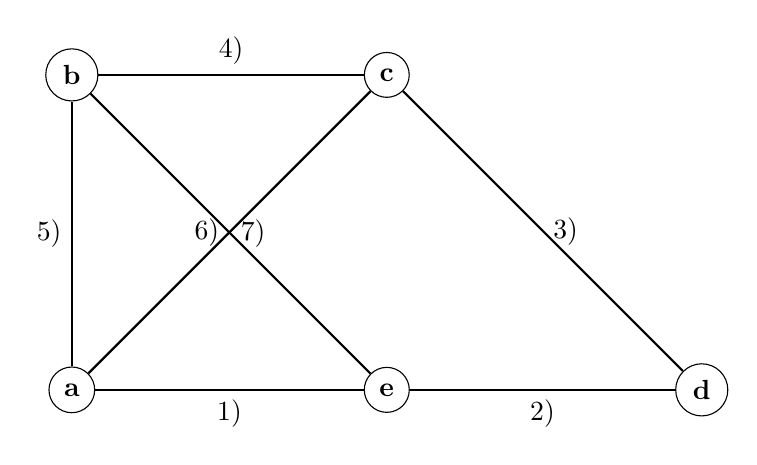
\begin{tikzpicture}
	
	\node[shape=circle,draw=black] (b) at (0, 4)     {\textbf{b}};
	\node[shape=circle,draw=black] (c) at (4, 4)     {\textbf{c}};
	\node[shape=circle,draw=black] (d) at (8, 0)     {\textbf{d}};
	\node[shape=circle,draw=black] (e) at (4, 0)     {\textbf{e}};
	\node[shape=circle,draw=black] (a) at (0, 0)     {\textbf{a}};
	
	\path[-, thick] (a) edge node[below]{1)}(e);
	\path[-, thick] (e) edge node[below]{2)}(d);
	\path[-, thick] (c) edge node[right]{3)}(d);
	\path[-, thick] (b) edge node[above]{4)}(c);
	\path[-, thick] (a) edge node[left]{5)} (b);
	\path[-, thick] (a) edge node[left]{6)}(c);
	\path[-, thick] (b) edge node[right]{7)}(e);
	
	\end{tikzpicture} 
	\caption{Graph G in Q1.}	
	\label{fig:g1}
\end{figure}

\subsection*{a) What is the sum of degrees of all nodes of G ?} 

	$-$ Degrees of a, b, c, e are 3 and the degree of d is 2. So, the sum of degrees of all nodes of G is $3+3+3+3+2 = 14$\\

\subsection*{b) What is the number of non-zero entries in the adjacency matrix representation of G ?} 

\begin{figure}[H]
            $$  
                \begin{bmatrix}{}
                     &\vline a & b & c & d & e \\ 
			\hline
		  a &\vline 0 & 1 & 1 & 0 & 1 \\
                  b &\vline 1 & 0 & 1 & 0 & 1 \\
                  c &\vline 1 & 1 & 0 & 1 & 0 \\
                  d &\vline 0 & 0 & 1 & 0 & 1 \\
		  e &\vline 1 & 1 & 0 & 1 & 0 \\
                \end{bmatrix}{} 
            $$
		\caption{The Adjacency Matrix Representation}
            \end{figure}{}
	$-$ The number of non-zero entries in the adjacency matrix representation of G is 14.\\

\subsection*{c) What is the number of zero entries in the incidence matrix representation of G ?} 

\begin{figure}[H]
            $$  
                \begin{bmatrix}{}
                      &\vline a & b & c & d & e \\ 
			\hline
		  1) &\vline 1 & 0 & 0 & 0 & 1 \\
                  2) &\vline 0 & 0 & 0 & 1 & 1 \\
                  3) &\vline 0 & 0 & 1 & 1 & 0 \\
                  4) &\vline 0 & 1 & 1 & 0 & 0 \\
		  5) &\vline 1 & 1 & 0 & 0 & 0 \\
 		  6) &\vline 1 & 0 & 1 & 0 & 0 \\
 		  7) &\vline 0 & 1 & 0 & 0 & 1 \\
                \end{bmatrix}{} 
            $$
		\caption{The Incidence Matrix Representation}
            \end{figure}{}

	$-$ The number of non-zero entries in the incidence matrix representation of G is 21.\\

\subsection*{d) Does G have a complete graph with at least four vertices as a subgraph ? If yes, give the subgraph.} 

	$-$ No, it doen't have a complete graph with at least four vertices as a subgraph. It has complete graphs with at least three vertices as a subgraph.\\

\subsection*{e) Is G bipartite ? Explain your answer.} 

	$-$ No, it isn't bipartite. A simple graph G is called bipartite if its vertex set $V$ can be partitioned into two disjoint sets $V_1$ and $V_2$ such that every edge in the graph connects a vertex in $V_1$ and a vertex in $V_2$.This means, the total number of edges that can be in a bipartite graph is $|V_1|*|V_2|$.\\
\\
	$-$ For the graph G, we can divide its vertices into groups of $(3-2), (2-3), (4-1), (1-4)$. So, the total number of edges there can be are (6, 6, 4, 4) for the combinations. However, there are 7 edges in the graph G. So, we can say that the graph G is not bipartite.\\
(Note: The representation $(a-b)$ means that size of $V_1 = a$ and size of $V_2= b$, and $|V_1|$ means the total number of vertices in $V_1$.)\\

\subsection*{f) How many directed graphs are there that have G as their underlying undirected graph ?}

	$-$ An edge of a directed graph can be in three different forms. It can be in the right or left direction. There are seven edges in the graph G.\\
	$-$ So, there can be $2^7$ different directed graphs that have G as their underlying undirected graph.\\

\subsection*{g) What is the length of the simple longest path in G? Give the path.}

	$-$ The length of the simple longest path in G is 4.\\
	$-$ The path is $(d,c,a,b,e)$. \\

\begin{figure}[H]
	\centering
	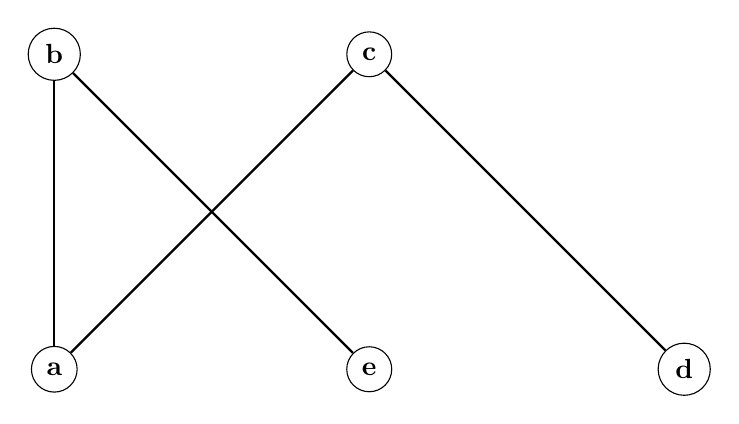
\begin{tikzpicture}
	
	\node[shape=circle,draw=black] (b) at (0, 4)     {\textbf{b}};
	\node[shape=circle,draw=black] (c) at (4, 4)     {\textbf{c}};
	\node[shape=circle,draw=black] (d) at (8, 0)     {\textbf{d}};
	\node[shape=circle,draw=black] (e) at (4, 0)     {\textbf{e}};
	\node[shape=circle,draw=black] (a) at (0, 0)     {\textbf{a}};
	
	
	\path[-, thick] (c) edge (d);
	\path[-, thick] (a) edge (b);
	\path[-, thick] (a) edge (c);
	\path[-, thick] (b) edge (e);
	
	\end{tikzpicture} 
	
\end{figure}

\subsection*{h) What is the number of connected components of G? Explain your answer.}

	$-$ The number of connected components of G is 1.\\
	$-$ A connected component of a graph G is a connected subgraph of G that is not a proper subgraph of another connected subgraph G. Forthe graph G, this subgraph is itself.\\ 

\subsection*{i) Is there an Euler circuit in G? If yes, give such a circuit; if no, state the reason.}

	$-$ No, there is not an Euler circuit in G. Let's assume that Euler circuit begins with a vertex a and continues with an edge incident with a. That edge contributes one to the degree of a. Each time the circuit passes through a vertex it contributes two to the vertex’s degree, because the circuit enters via an edge incident with this vertex and leaves via another such edge. In the end, the circuit comes to the node where it first started, in this case the node a, and increases the degree of a one more. Thus, to construct an  Euler circuit in a graph, every vertex must have a degree of even number. In the graph that is given to us, degrees of a, b, c, e are 3 and the degree of d is 2. So, we can't construct an Euler circuit.\\

\subsection*{j) Is there an Euler path in G? If yes, give such a path; if no, state the reason.}

	$-$ No, there is not an Euler path in G. When we travel on the graph, we will get stuck at some vertex x if that graph has more than 2 vertices of odd degree then we can conclude graphs like this has no Euler paths. In the graph that is given to us, degrees of a, b, c, e are 3 and the degree of d is 2. So, we can't construct an Euler path from it.\\

\subsection*{k) Does G have a Hamilton circuit? If yes, find such a circuit; if no, justify your answer.}

	$-$ There is a Hamilton circuit of G. $(a,b,c,d,e,a)$\\

\begin{figure}[H]
	\centering
	\begin{tikzpicture}
	
	\node[shape=circle,draw=black] (b) at (0, 4)     {\textbf{b}};
	\node[shape=circle,draw=black] (c) at (4, 4)     {\textbf{c}};
	\node[shape=circle,draw=black] (d) at (8, 0)     {\textbf{d}};
	\node[shape=circle,draw=black] (e) at (4, 0)     {\textbf{e}};
	\node[shape=circle,draw=black] (a) at (0, 0)     {\textbf{a}};
	
	\path[-, thick] (a) edge (e);
	\path[-, thick] (e) edge (d);
	\path[-, thick] (c) edge (d);
	\path[-, thick] (b) edge (c);
	\path[-, thick] (a) edge (b);
	%\path[-, thick] (a) edge node[left]{6)}(c);
	%\path[-, thick] (b) edge node[right]{7)}(e);
	
	\end{tikzpicture} 
	\caption{The Hamilton Circuit}
\end{figure}

\subsection*{l) Does G have a Hamilton path? If yes, find such a circuit; if no, justify your answer.}

	$-$ There is a Hamilton path of G. $(a,e,d,c,b)$

\begin{figure}[H]
	\centering
	\begin{tikzpicture}
	
	\node[shape=circle,draw=black] (b) at (0, 4)     {\textbf{b}};
	\node[shape=circle,draw=black] (c) at (4, 4)     {\textbf{c}};
	\node[shape=circle,draw=black] (d) at (8, 0)     {\textbf{d}};
	\node[shape=circle,draw=black] (e) at (4, 0)     {\textbf{e}};
	\node[shape=circle,draw=black] (a) at (0, 0)     {\textbf{a}};
	
	\path[-, thick] (a) edge (e);
	\path[-, thick] (e) edge (d);
	\path[-, thick] (c) edge (d);
	\path[-, thick] (b) edge (c);
	%\path[-, thick] (a) edge (b);
	%\path[-, thick] (a) edge node[left]{6)}(c);
	%\path[-, thick] (b) edge node[right]{7)}(e);
	
	\end{tikzpicture} 
	\caption{The Hamilton Path}
\end{figure}

\section*{Answer 2}
\begin{figure}[H]
	\centering
	\begin{subfigure}[b]{0.4\textwidth}
         \centering
         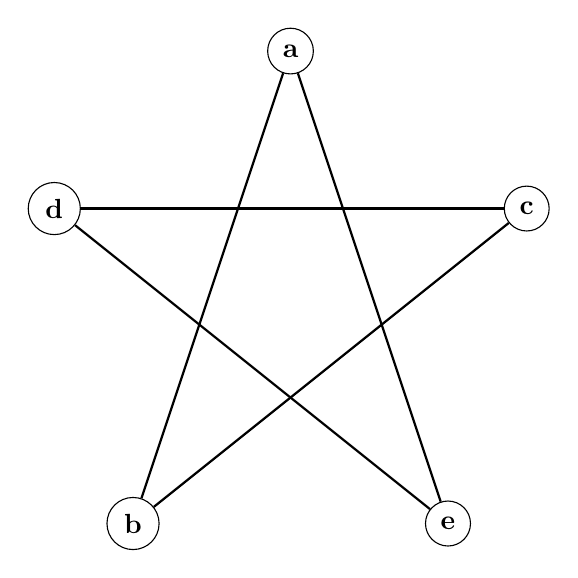
\begin{tikzpicture}
	
	\node[shape=circle,draw=black] (b) at (2, 0)     {\textbf{b}};
	\node[shape=circle,draw=black] (e) at (6, 0)     {\textbf{e}};
	\node[shape=circle,draw=black] (d) at (1, 4)     {\textbf{d}};
	\node[shape=circle,draw=black] (c) at (7, 4)     {\textbf{c}};
	\node[shape=circle,draw=black] (a) at (4, 6)     {\textbf{a}};
	
	\path[-, thick] (a) edge (b);
	\path[-, thick] (b) edge (c);
	\path[-, thick] (c) edge (d);
	\path[-, thick] (d) edge (e);
	\path[-, thick] (e) edge (a);
	
	\end{tikzpicture} 
         \caption{G}
         \label{fig:g}
     \end{subfigure}
     \hfill
     \begin{subfigure}[b]{0.4\textwidth}
         \centering
         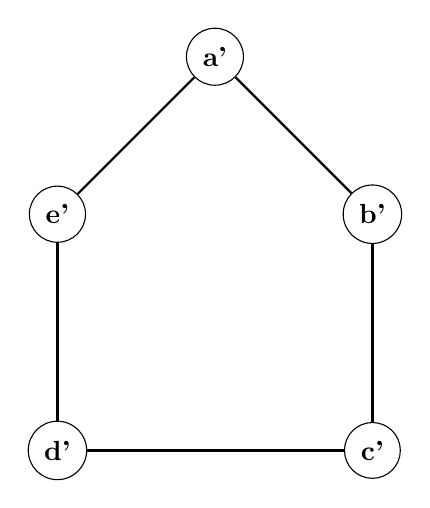
\begin{tikzpicture}
	
	\node[shape=circle,draw=black] (d') at (2, 0)     {\textbf{d'}};
	\node[shape=circle,draw=black] (c') at (6, 0)     {\textbf{c'}};
	\node[shape=circle,draw=black] (e') at (2, 3)     {\textbf{e'}};
	\node[shape=circle,draw=black] (b') at (6, 3)     {\textbf{b'}};
	\node[shape=circle,draw=black] (a') at (4, 5)     {\textbf{a'}};
	
    \path[-, thick] (a') edge (b');
    \path[-, thick] (a') edge (e');
    \path[-, thick] (b') edge (c');
    \path[-, thick] (d') edge (e');
    \path[-, thick] (c') edge (d');
	
	\end{tikzpicture} 
         \caption{H}
         \label{fig:h}
     \end{subfigure}
     \caption{Graph G and H in Q2.}
        \label{fig:g2}
\end{figure}

	Two graphs $G_1$ and $G_2$ said to be isomorphic if;\\
	\\
	$-$ Their number of components are the same.\\
	$-$ Their edge connectivity is retained.\\
	$-$ The degree of vertices are the same.\\
	$-$ Their adjacency matrices are the same.\\
	\\
	For the graphs in the question:\\
	$-$ Their number of components are the same. $(G = H =5)$\\
	$-$ Their edge connectivity is retained.\\
	$-$ The degree of vertices are the same. \\$(a=2, b=2, c=2, d=2, e=2)$ , $(a^{'}=2, b^{'}=2, c^{'}=2, d^{'}=2, e^{'}=2)$\\
	$-$ Their adjacency matrices are the same.\\

\begin{figure}[H]
            $$  
                \begin{bmatrix}{}
                     &\vline a & b & c & d & e \\ 
			\hline
		  a &\vline 0 & 1 & 0 & 0 & 1 \\
                  b &\vline 1 & 0 & 1 & 0 & 0 \\
                  c &\vline 0 & 1 & 0 & 1 & 0 \\
                  d &\vline 0 & 0 & 1 & 0 & 1 \\ 
		  e &\vline 1 & 0 & 0 & 1 & 0 \\
                \end{bmatrix}{} 
            $$
		\caption{The Adjacency Matrix Representation of G and H}
            \end{figure}{}




\section*{Answer 3}

\begin{figure}[H]
	\centering
	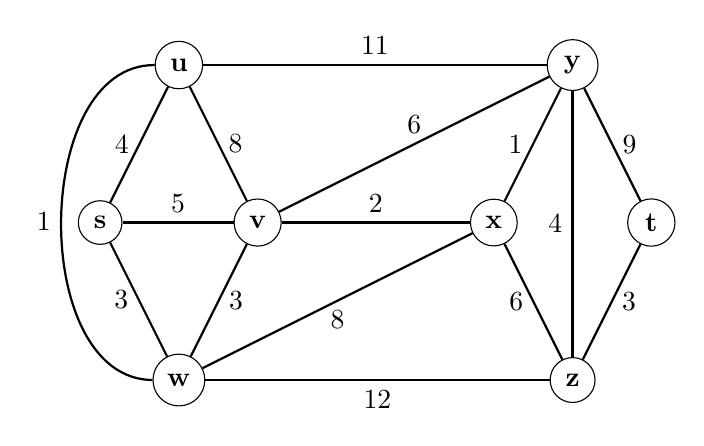
\begin{tikzpicture}
	
	\node[shape=circle,draw=black] (s) at (-1, 2)     {\textbf{s}};
	\node[shape=circle,draw=black] (u) at (0, 4)     {\textbf{u}};
	\node[shape=circle,draw=black] (y) at (5, 4)     {\textbf{y}};
	\node[shape=circle,draw=black] (w) at (0, 0)     {\textbf{w}};
	\node[shape=circle,draw=black] (z) at (5, 0)     {\textbf{z}};
	\node[shape=circle,draw=black] (v) at (1, 2)     {\textbf{v}};
        \node[shape=circle,draw=black] (x) at (4, 2)     {\textbf{x}};
        \node[shape=circle,draw=black] (t) at (6, 2)     {\textbf{t}};
 
	\path[-, thick] (u) edge [bend right=90] node[left]{1} (w);
	\path[-, thick] (s) edge node[left]{4} (u);
	\path[-, thick] (s) edge node[above]{5} (v);
	\path[-, thick] (u) edge node[right]{8} (v);
	\path[-, thick] (s) edge node[left]{3} (w);
	\path[-, thick] (v) edge node[right]{3} (w);
	\path[-, thick] (u) edge node[above]{11} (y);
	\path[-, thick] (y) edge node[right]{9} (t);
	\path[-, thick] (y) edge node[left]{1} (x);
	\path[-, thick] (y) edge node[left]{4} (z);
	\path[-, thick] (x) edge node[left]{6} (z);
	\path[-, thick] (t) edge node[right]{3} (z);
	\path[-, thick] (w) edge node[below]{12} (z);
	\path[-, thick] (x) edge node[below]{8} (w);
	\path[-, thick] (v) edge node[above]{2} (x);
	\path[-, thick] (v) edge node[above]{6} (y);
	
	\end{tikzpicture} 
	\caption{Graph G in Q3.}	
	\label{fig:g3}
\end{figure}

	The process we will follow:\\
	$-$ Vertex s is our starting vertex.\\
	$-$ Assign the infinity path values to all other vertices.\\
	$-$ Go to each vertex and update their path length.\\
	$-$ If the path length of the adjacent vertex is lesser than new path length, simply don't update.\\
	$-$ Avoid updating the path lengths of already visited vertices.\\
	$-$ After each iteration, pick the unvisited vertex with the least path length.\\
	$-$ Repeat until all the vertices have been visited.\\ 



\subsection*{step 1}
	$-$ Node s is the initial node. A node's distance to itself is 0. Set node s to 0 and all other nodes to $\infty$.\\

\subsection*{step 2}
	$-$ Visit node s. Set the distance values of the neighbours of s to the edge weight between them and s.\\
	\\
	$-$$u = 4 \implies (s \rightarrow u)$\\
	$-$$v = 5 \implies (s \rightarrow v)$\\
	$-$$w = 3 \implies (s \rightarrow w)$\\
	\\
	visited nodes: $s$\\

\subsection*{step 3}
	$-$ Visit the node with minimum distance value(w in this case). Update the x and z's distance values.\\
	\\
	$-$$u = 4 \implies (s \rightarrow u)$\\
	$-$$v = 5 \implies (s \rightarrow v)$\\
	$-$$w = 3 \implies (s \rightarrow w)$\\
	$-$$x = 11 \implies (s \rightarrow w \rightarrow x)$\\
	$-$$z = 15 \implies (s \rightarrow w \rightarrow z)$\\
	\\
	visited nodes: $(s-w)$\\

\subsection*{step 4}

	$-$ Visit the node u. Update y's distance value.\\
	\\
	$-$$u = 4 \implies (s \rightarrow u)$\\
	$-$$v = 5 \implies (s \rightarrow v)$\\
	$-$$w = 3 \implies (s \rightarrow w)$\\
	$-$$x = 11 \implies (s \rightarrow w \rightarrow x)$\\
	$-$$z = 15 \implies (s \rightarrow w \rightarrow z)$\\
	$-$$y = 15 \implies (s \rightarrow u \rightarrow y)$\\
	\\
	visited nodes: $(s-w-u)$\\

\subsection*{step 5}
	$-$ Visit the node v. Update x and y's distance values.\\
	\\
	$-$$u = 4 \implies (s \rightarrow u)$\\
	$-$$v = 5 \implies (s \rightarrow v)$\\
	$-$$w = 3 \implies (s \rightarrow w)$\\
	$-$$x = 7 \implies (s \rightarrow v \rightarrow x)$\\
	$-$$z = 15 \implies (s \rightarrow w \rightarrow z)$\\
	$-$$y = 11 \implies (s \rightarrow v \rightarrow y)$\\
	\\
	visited nodes: $(s-w-u-v)$\\

\subsection*{step 6}
	$-$ Visit the node with minimum distance value(x in this case). Update the y and z's distance values.\\
	\\
	$-$$u = 4 \implies (s \rightarrow u)$\\
	$-$$v = 5 \implies (s \rightarrow v)$\\
	$-$$w = 3 \implies (s \rightarrow w)$\\
	$-$$x = 7 \implies (s \rightarrow v \rightarrow x)$\\
	$-$$z = 13 \implies (s \rightarrow v \rightarrow x \rightarrow z)$\\
	$-$$y = 8 \implies (s \rightarrow v \rightarrow x \rightarrow y)$\\
	\\
	visited nodes: $(s-w-u-v-x)$\\

\subsection*{step 7}
	$-$ Visit the node with minimum distance value(y this time). Update the z and t's distance values.\\
	\\
	$-$$u = 4 \implies (s \rightarrow u)$\\
	$-$$v = 5 \implies (s \rightarrow v)$\\
	$-$$w = 3 \implies (s \rightarrow w)$\\
	$-$$x = 7 \implies (s \rightarrow v \rightarrow x)$\\
	$-$$z = 12 \implies (s \rightarrow v \rightarrow x \rightarrow y \rightarrow z)$\\
	$-$$y = 8 \implies (s \rightarrow v \rightarrow x \rightarrow y)$\\
	$-$$t = 17 \implies (s \rightarrow v \rightarrow x \rightarrow y \rightarrow t)$\\
	\\
	visited nodes: $(s-w-u-v-x-y)$\\

\subsection*{step 8}
	$-$ Visit the node with minimum distance value(z this time). Update t's distance value.\\
	\\
	$-$$u = 4 \implies (s \rightarrow u)$\\
	$-$$v = 5 \implies (s \rightarrow v)$\\
	$-$$w = 3 \implies (s \rightarrow w)$\\
	$-$$x = 7 \implies (s \rightarrow v \rightarrow x)$\\
	$-$$z = 12 \implies (s \rightarrow v \rightarrow x \rightarrow y \rightarrow z)$\\
	$-$$y = 8 \implies (s \rightarrow v \rightarrow x \rightarrow y)$\\
	$-$$t = 15 \implies (s \rightarrow v \rightarrow x \rightarrow y \rightarrow z \rightarrow t)$\\
	\\
	visited nodes: $(s-w-u-v-x-y-z)$\\

\subsection*{step 8}
	$-$ Visit the node t.\\
	\\
	$-$$u = 4 \implies (s \rightarrow u)$\\
	$-$$v = 5 \implies (s \rightarrow v)$\\
	$-$$w = 3 \implies (s \rightarrow w)$\\
	$-$$x = 7 \implies (s \rightarrow v \rightarrow x)$\\
	$-$$z = 12 \implies (s \rightarrow v \rightarrow x \rightarrow y \rightarrow z)$\\
	$-$$y = 8 \implies (s \rightarrow v \rightarrow x \rightarrow y)$\\
	$-$$t = 15 \implies (s \rightarrow v \rightarrow x \rightarrow y \rightarrow z \rightarrow t)$\\
	\\
	visited nodes: $(s-w-u-v-x-y-z-t)$\\

\subsection*{step 9}
	$-$ Dijktra's algorith has finished since there is no vertex left that is unvisited.\\
	\\
	$-$ In conclusion, the shortest path from s to t is $s \rightarrow v \rightarrow x \rightarrow y \rightarrow z \rightarrow t$ with the length of 15.\\

\begin{table}[H]
        \centering
        \begin{tabular}{|c|c|c|c|c|c|c|c|c|c|}
		\hline
                 & visited & s & u & v & w & x & y & z & t \\
             \hline
             step 1  & - & $0^{*}$ & $\infty$ & $\infty$ & $\infty$ & $\infty$ & $\infty$ & $\infty$ & $\infty$\\
             step 2  & s & $0^{*}$ &      4    &      5    &      3     & $\infty$ & $\infty$ & $\infty$ & $\infty$\\
             step 3  & w & $0^{*}$ &      4    &      5    & $3^{*}$ &     11    & $\infty$ &      15   & $\infty$\\
             step 4  & u & $0^{*}$ & $4^{*}$ &      5    & $3^{*}$ &   11    &     15    &     15    & $\infty$\\
             step 5  & v & $0^{*}$ & $4^{*}$ & $5^{*}$& $3^{*}$ &   7      & 11       & 15        & $\infty$\\
             step 6  & x & $0^{*}$ & $4^{*}$ & $5^{*}$ &  $3^{*}$ & $7^{*}$ & 8    &   13    & $\infty$\\
             step 7  & y & $0^{*}$ & $4^{*}$ & $5^{*}$ &  $3^{*}$ & $7^{*}$ & $8^{*}$ &  12  &   17\\
             step 7  & y & $0^{*}$ & $4^{*}$ & $5^{*}$ &  $3^{*}$ & $7^{*}$ & $8^{*}$ &  $12^{*}$ &15\\
		step 9  & t & $0^{*}$ & $4^{*}$ &  $5^{*}$  & $3^{*}$ & $7^{*}$ & $8^{*}$  & $12^{*}$ & $15^{*}$\\
		\hline
               
        \end{tabular}
        
	\caption{Note: * means visited}
	

    \end{table}{}



\section*{Answer 4}


\begin{figure}[H]
	\centering
	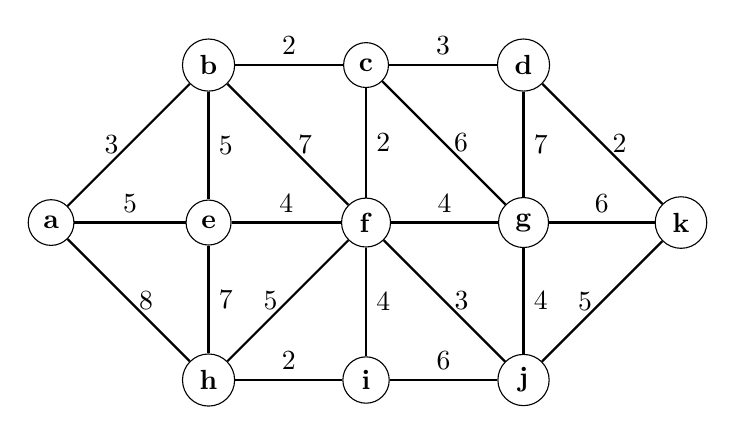
\begin{tikzpicture}
	
	\node[shape=circle,draw=black] (a) at (-2, 2)     {\textbf{a}};
	\node[shape=circle,draw=black] (b) at (0, 4)     {\textbf{b}};
	\node[shape=circle,draw=black] (c) at (2, 4)     {\textbf{c}};
	\node[shape=circle,draw=black] (d) at (4, 4)     {\textbf{d}};
	\node[shape=circle,draw=black] (e) at (0, 2)     {\textbf{e}};
	\node[shape=circle,draw=black] (f) at (2, 2)     {\textbf{f}};
	\node[shape=circle,draw=black] (g) at (4, 2)     {\textbf{g}};
	\node[shape=circle,draw=black] (h) at (0, 0)     {\textbf{h}};
	\node[shape=circle,draw=black] (i) at (2, 0)     {\textbf{i}};
	\node[shape=circle,draw=black] (j) at (4, 0)     {\textbf{j}};
	\node[shape=circle,draw=black] (k) at (6, 2)     {\textbf{k}};
	
	\path[-, thick] (a) edge node[left]{3} (b);
	\path[-, thick] (a) edge node[above]{5} (e);
	\path[-, thick] (a) edge node[right]{8} (h);
	\path[-, thick] (b) edge node[above]{2} (c);
	\path[-, thick] (b) edge node[right]{5} (e);
	\path[-, thick] (b) edge node[right]{7} (f);
	\path[-, thick] (c) edge node[above]{3} (d);
	\path[-, thick] (c) edge node[right]{2} (f);
	\path[-, thick] (c) edge node[right]{6} (g);
	\path[-, thick] (d) edge node[right]{7} (g);
	\path[-, thick] (d) edge node[right]{2} (k);
	\path[-, thick] (e) edge node[above]{4} (f);
	\path[-, thick] (e) edge node[right]{7} (h);
	\path[-, thick] (f) edge node[above]{4} (g);
	\path[-, thick] (f) edge node[left]{5} (h);
	\path[-, thick] (f) edge node[right]{4} (i);
	\path[-, thick] (f) edge node[right]{3} (j);
	\path[-, thick] (g) edge node[right]{4} (j);
	\path[-, thick] (g) edge node[above]{6} (k);
	\path[-, thick] (h) edge node[above]{2} (i);
	\path[-, thick] (i) edge node[above]{6} (j);
	\path[-, thick] (j) edge node[left]{5} (k);
	
	\end{tikzpicture} 
	\caption{Graph G in Q4.}	
	\label{fig:g4}
\end{figure}

\subsection*{a) Write the order in which the edges are added to the tree.} 
	We are going to use Kruskal's Algorithm. The process we will follow is:\\
	$-$ Sort all the edges in non-decreasing order.\\
	$-$ Pick the smallest edge.\\
	$-$ Check if it forms a cycle with the minimum spanning tree.\\
	$-$ If the cycle is not formed, add this edge, else discard it.\\
	$-$ Repeat until there are V-1 edges. (V is the number of vertices)\\

\begin{table}[H]
        \centering
        \begin{tabular}{c|c|c}
             Order & Edge & Weight \\
             \hline
             1  & \texttt{\{d,k\}} & 2 \\
             2  & \texttt{\{b,c\}} & 2 \\
             3  & \texttt{\{c,f\}} & 2 \\
             4  & \texttt{\{h,i\}} & 2 \\
             5  & \texttt{\{a,b\}} & 3 \\
             6  & \texttt{\{c,d\}} & 3 \\
             7  & \texttt{\{f,j\}} & 3 \\
             8  & \texttt{\{f,g\}} & 4 \\
             9  & \texttt{\{e,f\}} & 4 \\
             10 & \texttt{\{f,i\}} & 4
        \end{tabular}
        ~ \\
        ~ \\
        Total: 29
    \end{table}{}

\subsection*{b) Draw the minimum spanning tree.} 

\begin{figure}[H]
	\centering
	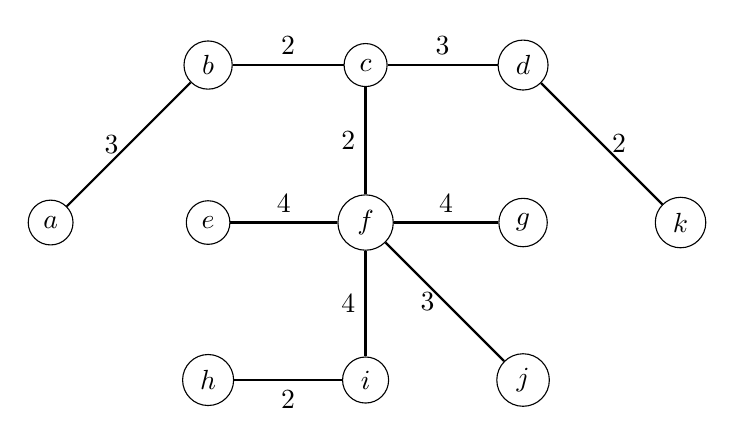
\begin{tikzpicture}
	\node[shape=circle,draw=black] (a) at (0, 2)     {\textbf{$a$}};
	\node[shape=circle,draw=black] (b) at (2, 4)     {\textbf{$b$}};
	\node[shape=circle,draw=black] (c) at (4, 4)     {\textbf{$c$}};
	\node[shape=circle,draw=black] (d) at (6, 4)     {\textbf{$d$}};
	\node[shape=circle,draw=black] (e) at (2, 2)     {\textbf{$e$}};
	\node[shape=circle,draw=black] (f) at (4, 2)     {\textbf{$f$}};
	\node[shape=circle,draw=black] (g) at (6, 2)     {\textbf{$g$}};
	\node[shape=circle,draw=black] (h) at (2, 0)     {\textbf{$h$}};
	\node[shape=circle,draw=black] (i) at (4, 0)     {\textbf{$i$}};
	\node[shape=circle,draw=black] (j) at (6, 0)     {\textbf{$j$}};
	\node[shape=circle,draw=black] (k) at (8, 2)     {\textbf{$k$}};


	\path[-, thick] (a) edge node[left]{3} (b);
	\path[-, thick] (b) edge node[above]{2} (c);
	\path[-, thick] (e) edge node[above]{4} (f);
	\path[-, thick] (h) edge node[below]{2} (i);	
	\path[-, thick] (c) edge node[above]{3} (d);
	\path[-, thick] (c) edge node[left]{2} (f);
	\path[-, thick] (f) edge node[left]{3} (j);
	\path[-, thick] (f) edge node[left]{4} (i);
	\path[-, thick] (d) edge node[right]{2} (k);
	\path[-, thick] (f) edge node[above]{4} (g);
	
	\end{tikzpicture}
\end{figure}

\subsection*{c) Is the minimum spanning tree unique? Justify your answer.} 

	$-$ Given a graph $G = (V,E)$ and a minimum spanning tree $M = (V,E_m)$\\
	\\
	If there exists an edge $e = (a,b) \in (E \setminus E_m)$ with weight $w(e) = x$ such that adding e to M will form a cycle C. Then if there exists another edge with the same weight with e in the cycle C, we can construct a second minimum spanning tree by swapping these two edges.\\
	\\
	For our graph, the edges $(f,g), (f,j), (g,j)$ forms a cycle. The weights of these edges are $(f,g) = 4, (f,j) = 3, (g,j) = 4$. Thus, we can construct another minimum spannig tree by swapping $(f,g)$ and $(g,j)$. So, the minimum spanning tree of our graph is not unique.\\

\begin{figure}[H]
	\centering
	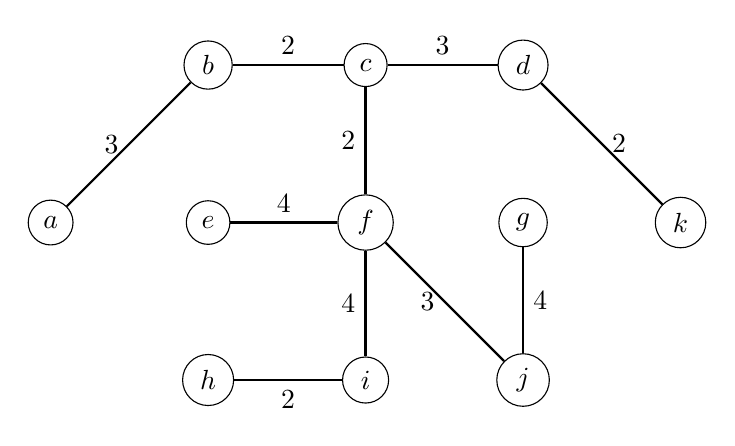
\begin{tikzpicture}
	\node[shape=circle,draw=black] (a) at (0, 2)     {\textbf{$a$}};
	\node[shape=circle,draw=black] (b) at (2, 4)     {\textbf{$b$}};
	\node[shape=circle,draw=black] (c) at (4, 4)     {\textbf{$c$}};
	\node[shape=circle,draw=black] (d) at (6, 4)     {\textbf{$d$}};
	\node[shape=circle,draw=black] (e) at (2, 2)     {\textbf{$e$}};
	\node[shape=circle,draw=black] (f) at (4, 2)     {\textbf{$f$}};
	\node[shape=circle,draw=black] (g) at (6, 2)     {\textbf{$g$}};
	\node[shape=circle,draw=black] (h) at (2, 0)     {\textbf{$h$}};
	\node[shape=circle,draw=black] (i) at (4, 0)     {\textbf{$i$}};
	\node[shape=circle,draw=black] (j) at (6, 0)     {\textbf{$j$}};
	\node[shape=circle,draw=black] (k) at (8, 2)     {\textbf{$k$}};


	\path[-, thick] (a) edge node[left]{3} (b);
	\path[-, thick] (b) edge node[above]{2} (c);
	\path[-, thick] (e) edge node[above]{4} (f);
	\path[-, thick] (h) edge node[below]{2} (i);	
	\path[-, thick] (c) edge node[above]{3} (d);
	\path[-, thick] (c) edge node[left]{2} (f);
	\path[-, thick] (f) edge node[left]{3} (j);
	\path[-, thick] (f) edge node[left]{4} (i);
	\path[-, thick] (d) edge node[right]{2} (k);
	\path[-, thick] (g) edge node[right]{4} (j);
	
	\end{tikzpicture}
	\caption{The Second MST}

\end{figure}






\end{document}